\section{Introduction}
\label{sec:Intro}

\IEEEPARstart{T}{he} recent advent of cloud computing has pushed the limits of data sharing capabilities for numerous applications that transcend geographical boundaries and involve millions of users. Governments and corporations today treat data sharing as a vital tool for enhanced productivity. Cloud computing has revolutionized education, healthcare and social networking. Perhaps the most exciting use case for cloud computing is its ability to allow multiple users across the globe share and exchange data, while saving the pangs of manual data exchanges, and avoiding the creation of redundant or out-of-date documents. Social networking sites have used the cloud to create a more connected world where people can share a variety of data including text and multimedia. Collaborative tools commonly supported by cloud platforms and are extremely popular since they lead to improved productivity and synchronization of effort. The impact of cloud computing has also pervaded the sphere of healthcare, with smpartphone applications that allow remote monitoring and even diagnosis of patients. In short, cloud computing is changing various aspects of our lives in unprecedented ways.

Despite all its advantages, the cloud is susceptible to privacy and security attacks, that are a major hindrance to its wholesome acceptance as the primary means of data sharing in today’s world. According to a survey carried out by IDC Enterprise Panel in August 2008 \cite{panelcloud}, Cloud users regarded security as the top challenge with $75\%$ of surveyed users worried about their critical business and IT systems being vulnerable to attack. While security threats from external agents are widespread, malicious service providers must also be taken into consideration. Since online data almost always resides in shared environments (for instance, multiple virtual machines running on the same physical device), ensuring security and privacy on the cloud is a non trivial task. When talking about security and privacy of data in the cloud, it is important to lay down the requirements that a data sharing service must provide in order to be considered secure. We list down here some of the most primary requirements that a user would want in a cloud-based data sharing service:

\begin{itemize}
 \item \emph{Data Confidentiality}: Unauthorized users (including the cloud service provider), should not be able to access the data at any given time. Data should remain confidential in transit, at rest and on backup media.
 
 \item \emph{User revocation}: The data owner must be able to revoke any user's access rights to data the without affecting other authorized users in the group. 
 
 \item \emph{Scalability and Efficiency}: Perhaps the biggest challenge faced by data management on the cloud is maintaining scalability and efficiency in the face of immensely large user bases and dynamically changing data usage patterns.
 
 \item \emph{Collusion between entities}: Any data sharing service in the cloud must ensure that even when certain malicious entities collude, they should still not be able to access any of the data in an unauthorized fashion. 

\end{itemize}

 
\begin{figure*}
\centering
\captionsetup{font=scriptsize}
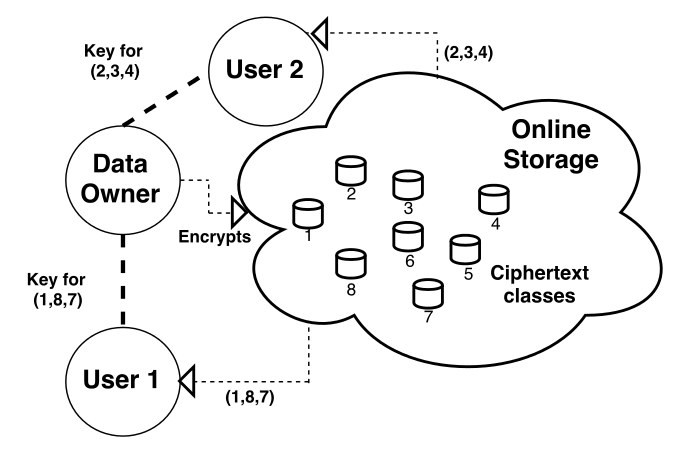
\includegraphics[scale=0.4]{Figs/KeyAgg.png}
\caption{Example of Online Data Sharing}
\label{fig:intro}
\end{figure*}

A traditional way of ensuring data privacy is to depend on the server to enforce access control mechanisms \cite{chow2012spice}. This methodology is prone to privilege escalation attacks in shared data environments such as the cloud, where data corresponding to multiple users could reside on the same server. Current technology for secure online data sharing comes in two major flavors - trusting a third party auditor \cite{cryptoeprint:2009:579}, or using the user's own key to encrypt her data while preserving anonymity \cite{chow2012dynamic}. In either case, a user would want a reliable and efficient cryptographic scheme in place, with formal guarantees of security, high scalability and ease of use. The main challenge in designing such a cryptosystem lies in effective sharing of encrypted data. A data sharing scheme on the cloud is only successful if data owners can delegate the access rights to their data efficiently to multiple users, who can then access the data directly from the cloud servers. Figure \ref{fig:intro} describes a realistic online data sharing set-up on the cloud. Assume that the data owner is using an online data sharing service such as Microsoft OneDrive \cite{shallman2014up} to store her research documents. She wishes to add an additional layer of security for her data by storing them in an encrypted fashion. Now, she intends to share specific subsets of these documents with different collaborators. For this, she needs to provide each of her collaborators with decryption rights to specific classes of the data that they are authorized to access. She might also wish to dynamically update the delegated access rights based on changes to the data/credibility issues. The challenge therefore is to provide her with a secure and efficient online \emph{partial} data sharing scheme that allows updates to user access rights on the fly.

A n\"{a}ive (and extremely inefficient) solution is to have a different decryption key for each ciphertext class, and share them accordingly with users via secured channels. This scheme is not practically deployable for two major reasons. Firstly, the number of secret keys would grow with the number of data classes. Secondly, any user revocation event would require Alice to entirely re-encrypt the corresponding subset of data, and distribute the new set of keys to the other existing valid users. This makes the scheme inefficient and difficult to scale. Since the decryption key in public key cryptosystems is usually sent via a secure channel, smaller key sizes are desirable. Moreover, resource constrained devices such as wireless sensor nodes and smart phones cannot afford large expensive storage for the decryption keys either. Not many of the present cryptosystems seem to address this issue of reducing the decryption key size for online data sharing schemes, as we describe next.


\subsection{Related Work}
\label{subsec:relatedwork}

In this section we present a brief overview of public and private key cryptographic schemes in literature for secure online data sharing. While many of them focus on key aggregation in some form or the other, very few have the ability to provide constant size keys to decrypt an arbitrary number of encrypted entities. One of the most popular techniques for access control in online data storage is to use a pre-defined hierarchy of secret keys in the form of a tree-like structure, where access to the key corresponding to any node implicitly grants access to all the keys in the subtree rooted at that node \cite{tzeng2002time,ateniese2012provably,sandhu1988cryptographic,sun2004scalable,atallah2009dynamic,ateniese2012provably}. A major disadvantage of hierarchical encryption schemes is that granting access to only a selected set of branches within a given subtree warrants an increase in the number of granted secret keys. This in turn blows up the size of the key shared. Compact key encryption for the symmetric key setting has been used in \cite{benaloh2009patient} to solve the problem of concisely transmitting  large number of keys in the broadcast scenario. However, symmetric key sharing via a secured channel is costly and not always practically viable for many applications on the cloud. Proxy re-encryption is another technique to achieve fine-grained access control and scalable user revocation in unreliable clouds \cite{ateniese2006improved,liu2011reliable}. However, proxy re-encryption essentially transfers the responsibility for secure key storage from the delegatee to the proxy and is susceptible to collusion attacks. It is also important to ensure that the transformation key of the proxy is well protected, and every decryption would require a separate interaction with the proxy, which is inconvenient for applications on the cloud.



% In this section we present a brief overview of public and private key cryptographic schemes in literature for secure online data sharing. While many of them focus on key aggregation in some form or the other, very few have the ability to provide constant size keys to decrypt an arbitrary number of encrypted entities.
% 
% \subsubsection{Hierarchical Encryption}
% \label{subsec:hierarchy}
% 
% One of the most popular techniques for access control in online data storage is to use a pre-defined hierarchy of secret keys \cite{akl1983cryptographic,chick1990flexible,tzeng2002time,ateniese2012provably} in the form of a tree-like structure, where access to the key corresponding to any node implicitly grants access to all the keys in the subtree rooted at that node. For instance, \cite{sandhu1988cryptographic} uses repeated evaluations of a pseudo-random function/block cipher on a fixed secret to generate a tree hierarchy of symmetric keys. Some more advanced schemes \cite{sun2004scalable,king2015centralized,atallah2009dynamic} extend access control to cyclic and acyclic graphs. A major disadvantage of hierarchical encryption schemes is that granting access to only a selected set of branches within a given subtree warrants an increase in the number of granted secret keys. This in turn blows up the size of the key shared. Thus while hierarchical cryptosystems provide a neat key delegation mechanism when 
% all files in a given branch is to be shared, its efficiency drops drastically as the complexity of the delegation increases.
% 
% \subsubsection{Compact Key Symmetric Encryption}
% \label{subsec:symmetric}
% 
% Compact key encryption for the symmetric key setting has been used in \cite{benaloh2009patient,benaloh2009key} to solve the problem of concisely transmitting  large number of keys in the broadcast scenario. The basic methodology is to divide the entire ciphertext space into a finite set of classes, followed by a constant size aggregate key generation for the set of classes to be delegated. This scheme thus solves the problem of multi-class delegation faced by hierarchical schemes. However, symmetric key sharing via a secured channel is costly and not always practically viable for many applications on the cloud. Some other schemes in the symmetric key setting also attempt to reduce the key size \cite{alomair2009information}, but they are not aimed at decryption key delegation and are hence not very relevant to the present discussion.
% 
% \subsubsection{Compact Key Identity-Based Encryption}
% \label{subsec:IBE}
% 
% Identity-Based Encryption (IBE) is a public key-based encryption scheme in which the public key for any user is an identity-string corresponding to that user. Proposed initially in \cite{shamir1985identity}, IBE was concretized by the proposition of two very widely cited and popular IBEs - The Boneh-Franklin scheme  \cite{boneh2003identity} and Cocks' encryption scheme \cite{cocks2001identity}. An IBE system comprises of a trusted private key generator that holds a master-secret key and issues a secret key to each user based on the user identity. Each user receives a message that has been encrypted using her id and some public parameters, and can decrypt the same using the secret key allotted to her by the trusted party. Compact key IBEs have been proposed in \cite{guo2007identity} and \cite{guo2008multi}. The former approach involves the use of random oracles while the latter shuns the use of oracles. Both these schemes allow aggregation of keys; however each key must come from a different identity division. Fuzzy IBE \cite{sahai2005fuzzy} allows for a single compact key to decrypt multiple ciphertexts, but they must have been encrypted under a closed set of identities, and the scheme does not work in practical scenarios for arbitrary identities. 
% 
% \subsubsection{Attribute Based Encryption}
% \label{subsec:ABE}
% 
% Attribute-based encryption (ABE) \cite{goyal2006attribute,bethencourt2007ciphertext,chase2007multi} allows each user to be identified by a set of attributes. An encrypted file stored in cloud can only be decrypted by an user who has access to the corresponding secret key. The secret key is securely transmitted to the user who satisfies the access control policies set by the data owner. A major drawback of this scheme is that each time the access right to a particular user is revoked the entire ciphertext has to be recrypted in the cloud. The idea of ABE has been extended to shared keys for user groups in \cite{li2013scalable} with the focus on collusion resistance and not on key size compression.  
% 
% \subsubsection{Proxy Re-Encryption}
% \label{subsec:PBE}
% 
% Proxy re-encryption is another technique to achieve fine-grained access control and scalable user revocation in unreliable clouds \cite{ateniese2006improved}. In this method the data owner and a semi trusted proxy cloud share a secret key in advance, with which the cloud can be delegated to re-encrypt data on behalf of the data owner. The semi-trusted proxy re-encrypts the data using the data owner's public key, thus converting it into a file that can in turn be decrypted by the secret key of the client. In the whole process, the proxy has no knowledge of the data being sent. An extension to this technique has been proposed in \cite{liu2011reliable} that allows the cloud servers to automatically re-encrypt data based on their internal clocks, without any external trigger. However, proxy re-encryption essentially transfers the responsibility for secure key storage from the delegatee to the proxy and is susceptible to collusion attacks. It is also important to ensure that the transformation key of the proxy is well protected, and every decryption would require a separate interaction with the proxy, which is inconvenient for applications on the cloud.


\subsection{The Key-Aggregate Encryption Scheme}
\label{subsec:KAC_orig}

The most efficient proposition pertaining to our problem statement, to the best of our knowledge, is made in \cite{chu2014key}. The proposition is to allow Alice to combine the decryption power of multiple data classes into a single key of constant size. Thus, while each class of data is encrypted using a different public key, a single decryption key of constant size is sufficient to decrypt any subset of these classes. This system is popularly known as the key-aggregate cryptosystem~(KAC), and derives its roots from the seminal work by Boneh \textit{et.al.} \cite{boneh2005collusion} that allows broadcasting of data (encrypted by the same public key) among multiple users, each of whom possess their own private keys for decryption. In KAC, when a user demands for a particular subset of the available classes of data, the data owner computes an aggregate key which integrates the power of the individual decryption keys corresponding to each class of data. However, KAC as proposed in \cite{chu2014key} suffers from two major drawbacks, each of which we address in this paper. 


\begin{enumerate}

 \item Firstly, no concrete proofs of cryptographic security for KAC are provided by the authors of \cite{chu2014key}. Formal proofs are considered to be of paramount importance in establishing the security of any cryptographic scheme, since they define the specific adversarial models against which the scheme is secure. 
 
 \item Secondly, the scheme proposed in \cite{chu2014key} does not explicitly address the issue of aggregate key distribution among multiple users. In a practical data sharing environment with millions of users, it is neither practical nor efficient to depend on the existence of secure channels for key distribution. A public key based solution for broadcasting the aggregate key among an arbitrarily large number of users is hence desirable.
\end{enumerate}

 
 
\subsection{Our Contributions}
\label{subsec:contributions}

The main contributions of this paper can be enumerated as follows:
\begin{enumerate}

 \item In this paper we propose an efficient key-aggregate cryptosystem (KAC) for online data sharing on the cloud using efficiently implementable asymmetric bilinear pairings.
 
 \item We further generalize the basic KAC construction using a two-tier scheme and demonstrate how this allows multiple data owners to share their data while enjoying full data privacy.
 
 \item We demonstrate how the basic KAC framework may be efficiently extended for securely broadcasting the aggregate key among multiple data users in a real-life data sharing environment. This in turn allows us to build a fully public-key based online data sharing scheme that is highly scalable.
 
 \item All our constructions are fully collusion resistant and are proven to be statically CPA and CCA secure under different complexity assumptions.
 
 \item Implementation details and simulation results demonstrate that our proposed construction actually scales better than traditional hierarchical cryptosystems in terms of space and time complexity requirements.
 
\end{enumerate}



 









